\documentclass{article}
\usepackage[utf8]{inputenc}
\usepackage{graphicx}
\graphicspath{ {images/} }

\title{Insertion Sort vs. Merge Sort}
\author{Vivoli Emanuele }
\date{28 April 2017}
\usepackage{algorithm}
\usepackage{algorithmic}

\begin{document}

\maketitle

\section{Introduzione}
Il prolema questa volta non è più l'ordinamento di un vettore o di una sequenza numerica, ma si tratta di confrontare i vari algoritmi di ordinamento visti nel corso (in particolare Insertion Sort e Merge Sort).

\section{Analisi}
\subsection{Insertion Sort}
Nell'analisi di Insertion Sort viene definito tj = #esecuzioni del confronto del while per un certo indice j.
Si vede dunque che il costo T(n) di Insertion Sort dipende dalla variabile definita tj, che dipende dagli input.
Dunque in base alla sequenza di input si valutano i seguenti casi:
\begin{description}

        \item[Caso migliore] Array gia ordinato e tj = 1 
        
        $T(n)= an + b$ ; a,b costanti. Funzione lineare di n
        
        \item[Caso peggiore] Array gia ordinato inversamente, e tj = j
        
        $T(n)= an^2 + bn + c$ ; 
        
        a,b,c sono costanti. Funzione quadratica di n.
        
        \item[Caso medio] In media A[j] metà degli elementi in A[1...j-1], e tj = j/2
        
        $T(n)= an^2 + bn + c$ ; 
        
        a,b,c costanti; indicativamente le costanti sono di valore metà di quelle nel caso peggiore. Funzione quadratica di n.
\end{description}
    
\subsection{Merge Sort}
L'algoritmo Merge Sort, per ordinare una sequenza di n oggetti, ha complessità temporale $T(n)=\Theta (n\log n)$ sia nel caso medio che nel caso pessimo. Infatti:

La funzione merge qui presentata ha complessità temporale  $\Theta (n)$,
mergesort richiama se stessa due volte, e ogni volta su (circa) metà della sequenza in input


Da questo segue che il tempo di esecuzione dell'algoritmo è dato dalla ricorrenza: $T(n)=2T\left({\frac  {n}{2}}\right)+\Theta (n)$ la cui soluzione in forma chiusa è $\Theta (n\log n)$, per il secondo caso del teorema dell'esperto.
Dunque si hanno i seguenti casi:
\begin{description}

        \item[Caso migliore] $\Theta (n\log n)$
        
        \item[Caso peggiore] $\Theta (n\log n)$
        
        \item[Caso medio] $\Theta (n\log n)$
        
\end{description}
Sappiamo, dopo averne visto anche il teorema e la dimostrazione, che un algoritmo che ordina per confronti ha un limite inferiore di confronti per il caso peggiore di $\Omega (nlgn)$, e cio' ci dice proprio che Merge Sort è un algoritmo di ordinamento per confronti asintoticamente ottimale poiche il limite superiore $O(nlgn)$ sui tempi di esecuzione corrisponde al limite inferiore $\Omega (nlgn)$ nel caso peggiore.

\section{Array 100 elementi}
\begin{center}
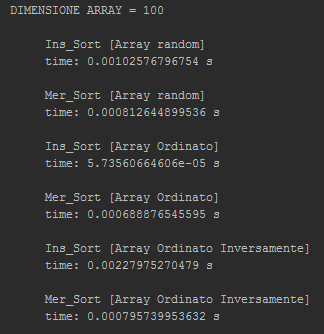
\includegraphics{photo100.png}
\end{center}

Possiamo notare da quest'esempio i tempi di esecuzione di Insertion Sort e Merge Sort su array di dimensione 100 elementi, ma con caratteristiche differenti. Nella prima esecuzione i 100 elementi dell'array sono generati randomicamente, ed i tempi di esecuzione di Insertion Sort e Merge Sort sono relativamente simili rispetto alla dimensione dell'array che trattiamo. Una notevole differenza la vediamo quando per Insertion Sort i valori dell'array sono gia ordinati, dove quindi il tempo di esecuzione decresce fortemente, mentre per Merge Sort sono (sempre con approssimazioni) uguali. Riguardo al caso peggiore di Insertion Sort non notiamo troppe differenze.



\section{Array 1000 elementi}
\begin{center}
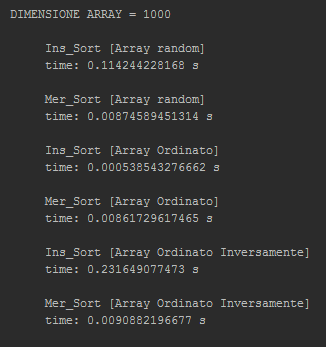
\includegraphics{photo1000.png}
\end{center}
In questo caso possiamo notare la differenza tra l'esecuzione di Insertion Sort nel caso migliore (Array ordinato) e la sua esecuzione nel caso medio e peggiore, notando come invece i tempi di Merge Sort restino (piu o meno) i soliti.

\section{Array 10000 elementi}
\begin{center}
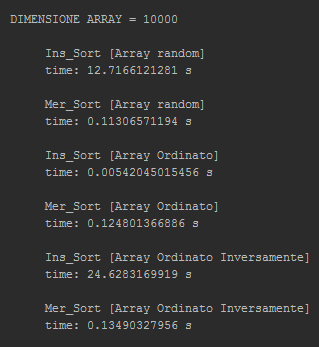
\includegraphics{photo10000.png}
\end{center}

In questo caso le differenza di esecuzine (seppur notevoli anche nelle esecuzioni precedenti con array di dimensione 100 e 1000) sono molto tangibili, dove notiamo fortemente che il caso di array ordinato in senso decrescente rappresenta il caso peggiore per Insertion Sort come avevamo definito nell'analisi precedente, che risolve l’ordinamento in $\Theta(n^2)$. Si vede quindi come anche in un array relativamente piccolo l’Insertion-Sort impiega molti secondi mentre il Merge-Sort non viene influenzato da questa particalare permutazione.
Nel caso dell’array ordinato si può vedere come l’Insertion Sort si rivela
essere la scelta migliore, infatti,il caso di array già ordinato,rappresenta
il caso ottimo e lo risolve in $\Theta(n)$. 

\section{Array 100000 elementi}
\begin{center}
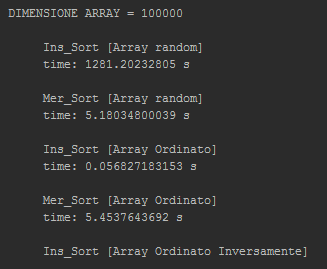
\includegraphics{photo100000.png}
\end{center}

In questo esempio possiamo notare come Insertion Sort impiega un tempo spropositato in confronto alla manciata di secondi con cui Merge Sort ordina un array di queste dimensioni. Il caso peggiore di Insertion Sort (Array ordinato inversamente) non viene risolto nemmeno dopo piu' di 15 minuti.

\end {document}